\chapter{SelB-k-NN: Replacing the Inefficient Operations}
\label{sec_3}

In this chapter, we discuss the first optimization approach with the example of SelB-\textit{k}-NN. Sec 3.1 discusses the background and motivation of the algorithm. Sec 3.2 introduces the central part of the single-core SelB-\textit{k}-NN algorithm. Sec 3.3 proposes two significant methods to minimize the hardware support requirements of the algorithm. In Sec 3.4, we discuss how we can quantify and achieve the optimized tiling shapes for large datasets. Sec 3.5 evaluates the performance of SelB-\textit{k}-NN, and Sec 3.6 concludes this chatper.

\section{Background \& Motivation}

\subsection{\textit{K}-Nearest Neighbors Algorithm}

\textit{K}-NN is one of the most classical and well-studied algorithms for classification problems. The general idea of \textit{k}-NN is uncomplicated: those points in the same category mostly have high similarity and are located close to one another in high-dimensional space. To classify a test point, \textit{k}-NN computes the similarity between the test point and all the training points and then selects the \textit{k} nearest neighbors in the \textit{k}-selection phase. \textit{K}-NN finally chooses the category of the most neighbors in the \textit{k} nearest neighbor results as the test point's category.

In the early days, the distance computation took most of the \textit{k}-NN's execution time. With the improvement of the hardware, GPUs with massive parallelism successfully mitigate the bottleneck. The \textit{k}-selection phase remains a new bottleneck with several solutions. In general, the \textit{k}-selection algorithms are divided into two categories, heap-based \cite{DBLP:conf/medi/VelentzasVC21, DBLP:conf/sigmod/ShanbhagPM18, DBLP:conf/ccgrid/KatoH10, DBLP:journals/concurrency/KatoH12, DBLP:conf/icip/GarciaDNB10, DBLP:conf/egh/LiSPAOA12} and bitonic-based \cite{DBLP:conf/sigmod/ShanbhagPM18, DBLP:journals/tbd/JohnsonDJ21, DBLP:conf/ipps/Tang0EMG15}. However, the two approaches rely on a considerable number of weakly supported operations on the AI processors. For 16-selection of 16 test points with 4096 training points on the Huawei Ascend 310 processors, the dynamic addressing during sibling selections in the re-heap procedure occupies 94.10\% of the heap-based \textit{k}-selection execution time. The vectorized comparisons \& selections, which support compare-and-swap operations, occupy 75.98\% of the bitonic-based \textit{k}-selection. A novel algorithm to reduce these operations on the AI processors is urgently needed.

\subsection{Tiling Shape Mismatch of \textit{K}-NN \label{sec:tiling}}

Tiling is an effective technique for matrix multiplication optimization, which benefits from the data locality and is widely studied on the different platforms including the AI processors \cite{DBLP:conf/ppopp/Li0YJL19, DBLP:conf/ppopp/NiuLJS0022, DBLP:conf/ppopp/HongSNSS19, DBLP:conf/ipps/00020C20, DBLP:conf/ppopp/FengWCZ0D21, DBLP:conf/micro/ZhaoD20}. It combines sufficient knowledge of the hardware structures and the fixed specific matrix multiplication execution patterns for maximized hardware performance.

However, most of their works separate the matrix multiplications from the applications. While the matrix multiplications prefer regular tiling shapes ($m \approx n$) on the Matrix MACs \cite{DBLP:conf/ipps/00020C20}, \textit{k}-selections prefer irregular ones ($m \gg n$) on the vector units, which brings a tiling shape mismatch. For example, the heap-based \textit{k}-selection is expanded efficiently along the $m$-direction, maintaining $m$ heaps on the vector units for parallel element-wise comparison. Increasing $m$ would not prolong the execution time seriously, while increasing $n$ raises the loop iterations and makes the execution longer. However, the matrix multiplication output restricts the $k$-selection's tiling shape. When selecting a regular tiling shape for the matrix multiplication, the relation $m \gg n$ cannot be true for the \textit{k}-selection. On other platforms, selecting the regular tiling shapes for $k$-NN may perform well. On AI processors, the matrix multiplication does not dominate the $k$-NN execution time. Directly applying matrix multiplication's tiling shapes works poorly on the $k$-selection and harms the $k$-NN performance.


\section{SelB-k-NN Algorithm}

\begin{figure}[t]
    \centering{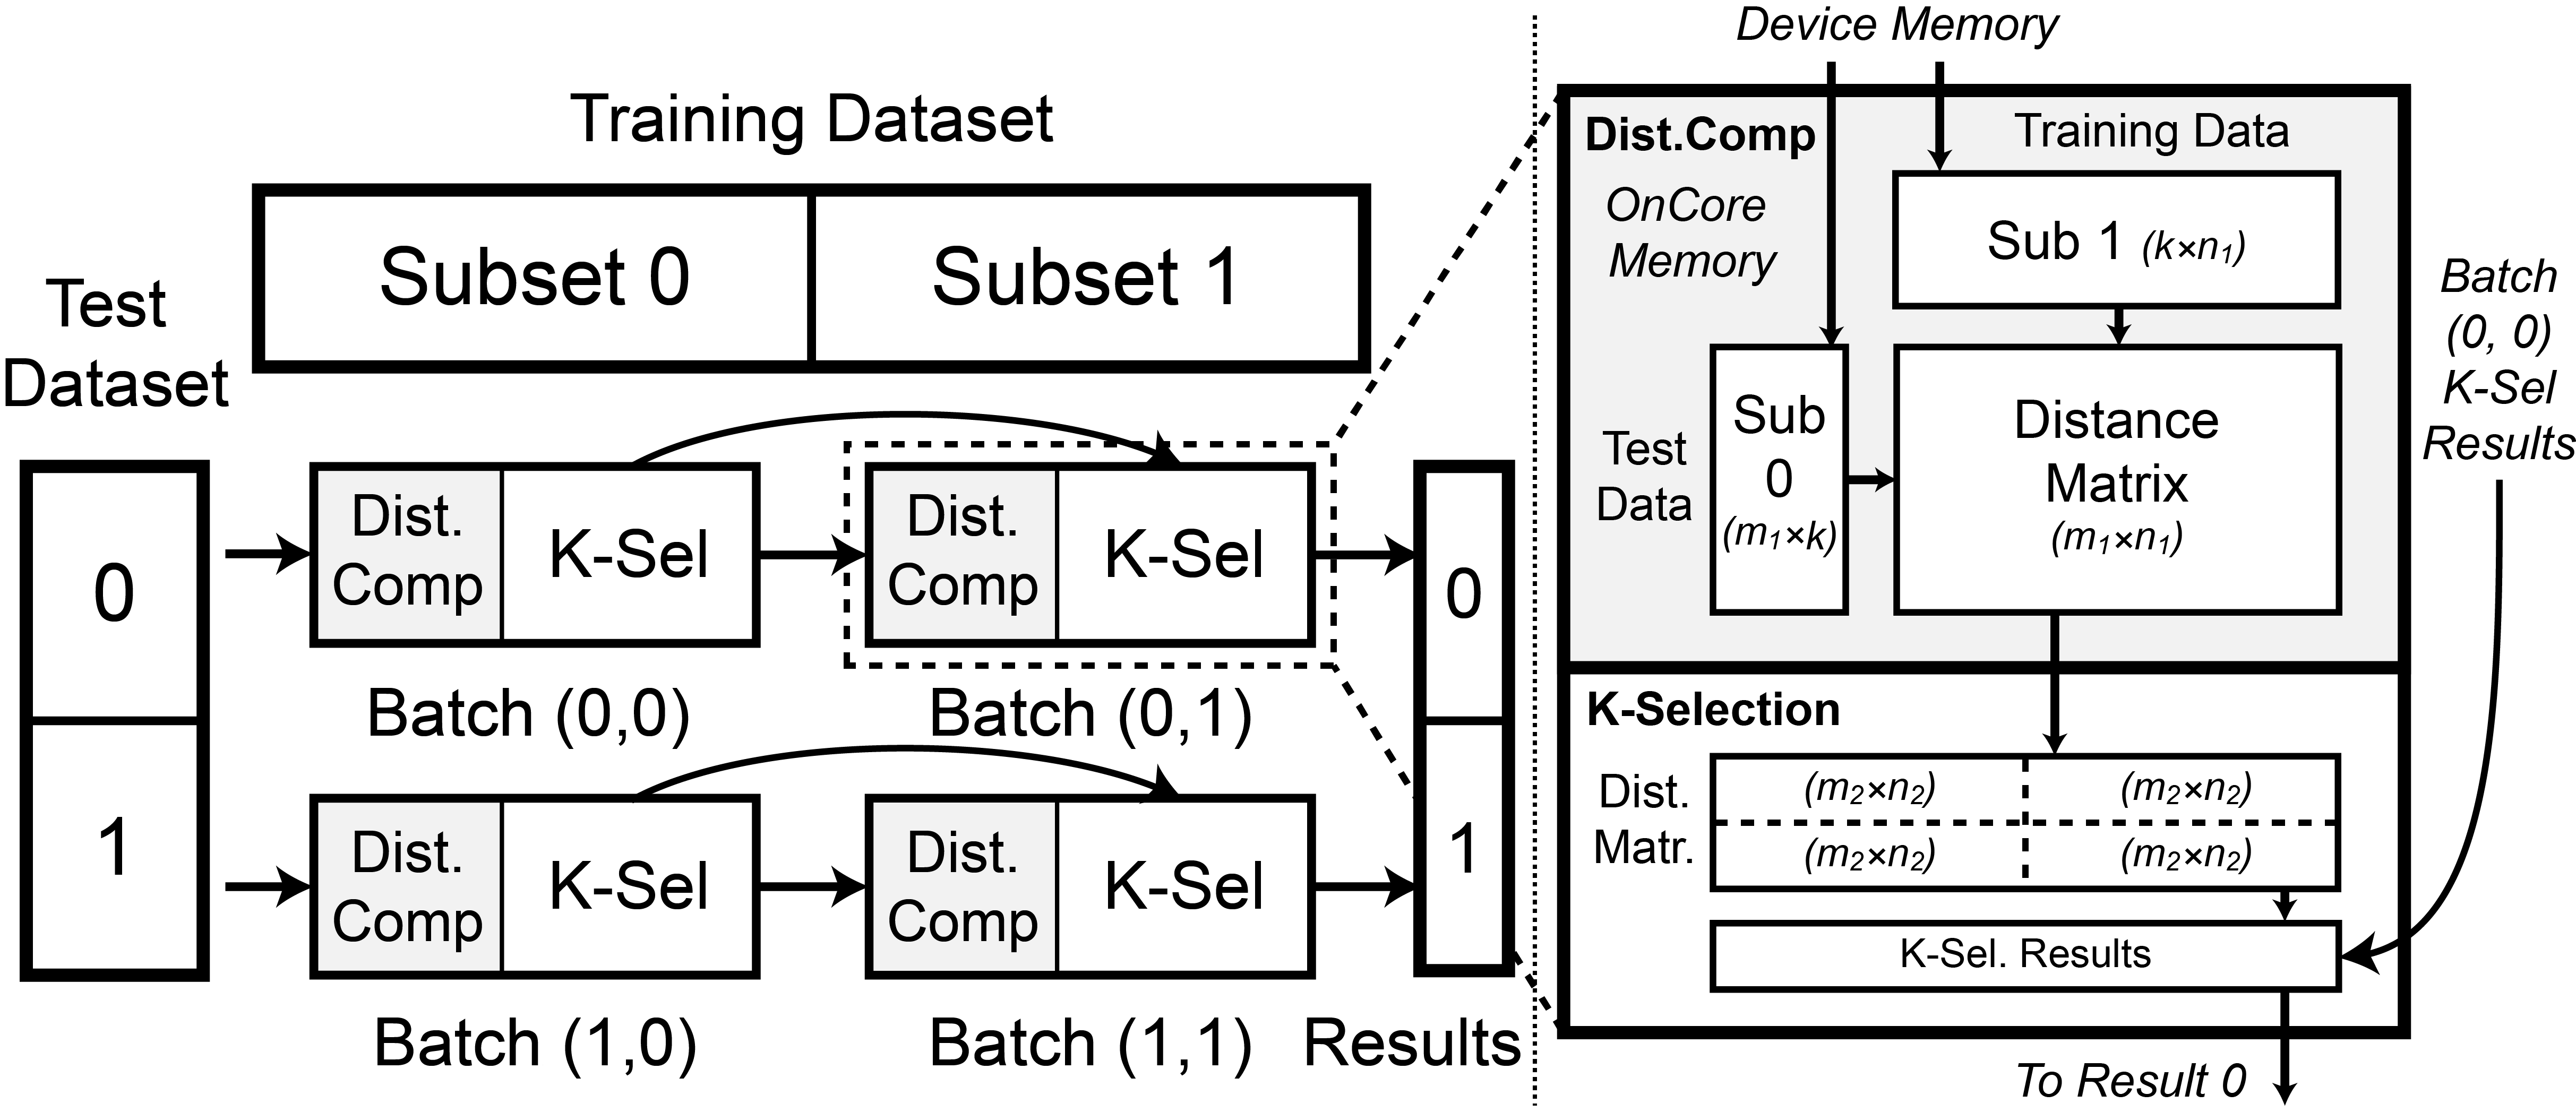
\includegraphics[scale=0.3]{figures/tiling.png}}
    \caption{An overview of SelB-\textit{k}-NN with a detailed view of the batch (0, 1)}
    \label{fig:tiling}
    \end{figure}

Fig. \ref{fig:tiling} illustrates an overview of SelB-\textit{k}-NN. It first tiles the test and training datasets along the $m$-direction and $n$-direction respectively. A batch is assigned a tile of the workload with the distance computation tiling shape $(m_1, n_1)$. It receives data from the datasets, computes and updates the previous min-\textit{k} results from the last adjacent batch along the $n$-direction. The \textit{k}-selection of each batch is further tiled with the tiling shape $(m_2, n_2)$, as shown on the right side of Fig. \ref{fig:tiling}. The processed data of each batch is transferred from the large but slow device memory, while the intermediate min-\textit{k} results can be maintained constantly at the fast but tiny on-core memory until the finish of the current test dataset tile along the $m$-direction. The mini-batches are executed sequentially on a single processor and easily applied to multi-processors \cite{van2007superlinear}. This section mainly describes a single batch of SelB-\textit{k}-NN.

\subsection{Distance Computation on AI Processors}

By accelerating the matrix multiplications with the Matrix MACs, the AI processors efficiently improve the performance of cosine distance computations. 

The cosine distance of points $\boldsymbol{p}_{1}, \boldsymbol{p}_{2}$ is:

\begin{equation}
    \label{eq:cosine}
    \begin{aligned}
    D_{cos} = 1 - \frac{\boldsymbol{p}_{1} \cdot \boldsymbol{p}_{2}}
            {\left\| \boldsymbol{p}_{1} \right\| 
                \left\| \boldsymbol{p}_{2} \right\|}
        = 1 - \boldsymbol{p}_{1} \cdot \boldsymbol{p}_{2}\  (\textnormal{for } \ell\textnormal{2-norm pts.})
    \end{aligned}
    \end{equation}

Therefore, the essence of the distance computation is the dot product of two vectors. For $m_1 \times n_1$ data, we compute the dot products following the matrix multiplication below:

\begin{equation}
    \label{eq:dot_products}
    \begin{aligned}
    \begin{bmatrix} 
        \boldsymbol{p}_{1} \\
        \vdots \\
        \boldsymbol{p}_{m_1}
    \end{bmatrix}
    \cdot
    \begin{bmatrix} 
        \boldsymbol{q}_{1}^{T} &
        \dots &
        \boldsymbol{q}_{n_1}^{T}
    \end{bmatrix}
    =
    \begin{bmatrix} 
        \boldsymbol{p}_{1} \cdot \boldsymbol{q}_{1} &
        \dots &
        \boldsymbol{p}_{1} \cdot \boldsymbol{q}_{n_1} \\
        \vdots & \ddots & \vdots \\
        \boldsymbol{p}_{m_1} \cdot \boldsymbol{q}_{1} &
        \dots &
        \boldsymbol{p}_{m_1} \cdot \boldsymbol{q}_{n_1} \\
    \end{bmatrix}
    \end{aligned}
    \end{equation}

where $\boldsymbol{p}_{i}$ and $\boldsymbol{q}_{i}$ are $d$ dimensional vectors. For simplicity, we assume that all the data in this work are $\ell$2-normalized, and the term \textit{distance} in the chapter is cosine distance.

\subsection{\textit{K}-Selection on AI Processors}

SelB-\textit{k}-NN \textit{k}-selection algorithm relies on two groups of common vectorized operations, which are used in the most significant operations in DNN applications and supported by AI processors \cite{CANN, jax, cambricon}. The first includes \verb|reduceMin| (and \verb|reduceMax|), which find the minimized value in a given vector. Some AI processors further support returning the corresponding indices \cite{CANN}. The two operations form the central part of the pooling layer, frequently used after convolutional layers. The other includes \verb|vecCmp| and \verb|vecSel|, which compare two given vectors by elements to build a mask and select the elements based on the mask. The two operations support an elementary branch for data, which is necessary for training like the backpropagation computation of \verb|ReLU|. However, as discussed, existing works \cite{DBLP:conf/icpp/JiW21, cambricon, CANN} indicate inefficiency or lack of the two operations on some AI processors.

Our \textit{k}-selection algorithm finds indices of the min-\textit{k} results for $m_2$ separate $n_2$-sized vectors in at most $k$ steps. For each vector, the general idea is to ensure that after the \textit{k}-selection phase, the minimum value remaining in the vector is greater than the maximum value in the min-\textit{k} results. Based on the idea, we propose the \textit{k}-selection algorithm in Alg. \ref{alg:single_main}.

\begin{algorithm}[tbp]
    \caption{SelB-\textit{k}-NN \textit{K}-Selection Algorithm}
    \label{alg:single_main}
        
    \SetKwInOut{Input}{Input}
    \SetKwInOut{Output}{Output}
        
    \Input{
        distance matrix \textbf{D} of size ($\textit{m}_2 \times \textit{n}_2$) \\
        last min-$k$ results \textbf{K} of size ($\textit{k} \times \textit{m}_2$) \\
        last indices of results \textbf{I} of size ($\textit{k} \times \textit{m}_2$)
    }
            
    \Output{
        min-$k$ results \textbf{K}$^{\prime}$ of size ($\textit{k} \times \textit{m}_2$) \\
        indices of results \textbf{I}$^{\prime}$ of size ($\textit{k} \times \textit{m}_2$)
    }
    \BlankLine
    
    $mask \leftarrow$ $\vec{\textbf{0}}$ \\
        
    \For{$step \leftarrow 0$ \KwTo $k$}{
        \For{$ln \leftarrow 0$ \KwTo $m$}{
            \If{$mask[ln] \neq 0$}{
                \textbf{continue}
            }
            $(res_{min}, idx_{min})[ln] \leftarrow$ \textbf{reduceMin}$(\textbf{D}[ln])$ \\
            $\textbf{D}[ln][idx_{min}[ln]] \leftarrow +\infty$ \tcp*{Scalar}
        }
        $cmp \leftarrow$ \textbf{vecCmpLt}$(res_{min}, \textbf{K}[0])$ \tcp*{Cmp}
        $mask \leftarrow$ \textbf{vecSel}$(cmp, mask, \vec{\textbf{1}})$ \tcp*{Sel}
        $mask_{min} \leftarrow$ \textbf{reduceMin}$(mask)$ \\
        \If{$mask_{min} \neq 0$}{
            \Return \textbf{K} as \textbf{K}$^{\prime}$, \textbf{I} as \textbf{I}$^{\prime}$
        }
        $\textbf{K}[0] \leftarrow$ \textbf{vecSel}$(cmp, res_{min}, \textbf{K}[0])$ \tcp*{Sel}
        $\textbf{I}[0] \leftarrow$ \textbf{vecSel}$(cmp, idx_{min}, \textbf{I}[0])$ \tcp*{Sel}
        $\textbf{bitonicKSel}(\textit{k} = 1, (\textbf{K}, \textbf{I}))$ \tcp*{O(\textit{k}) Cmp\&Sel}
    }
    \Return \textbf{K} as \textbf{K}$^{\prime}$, \textbf{I} as \textbf{I}$^{\prime}$
\end{algorithm}

\begin{figure}[tbp]
    \centering{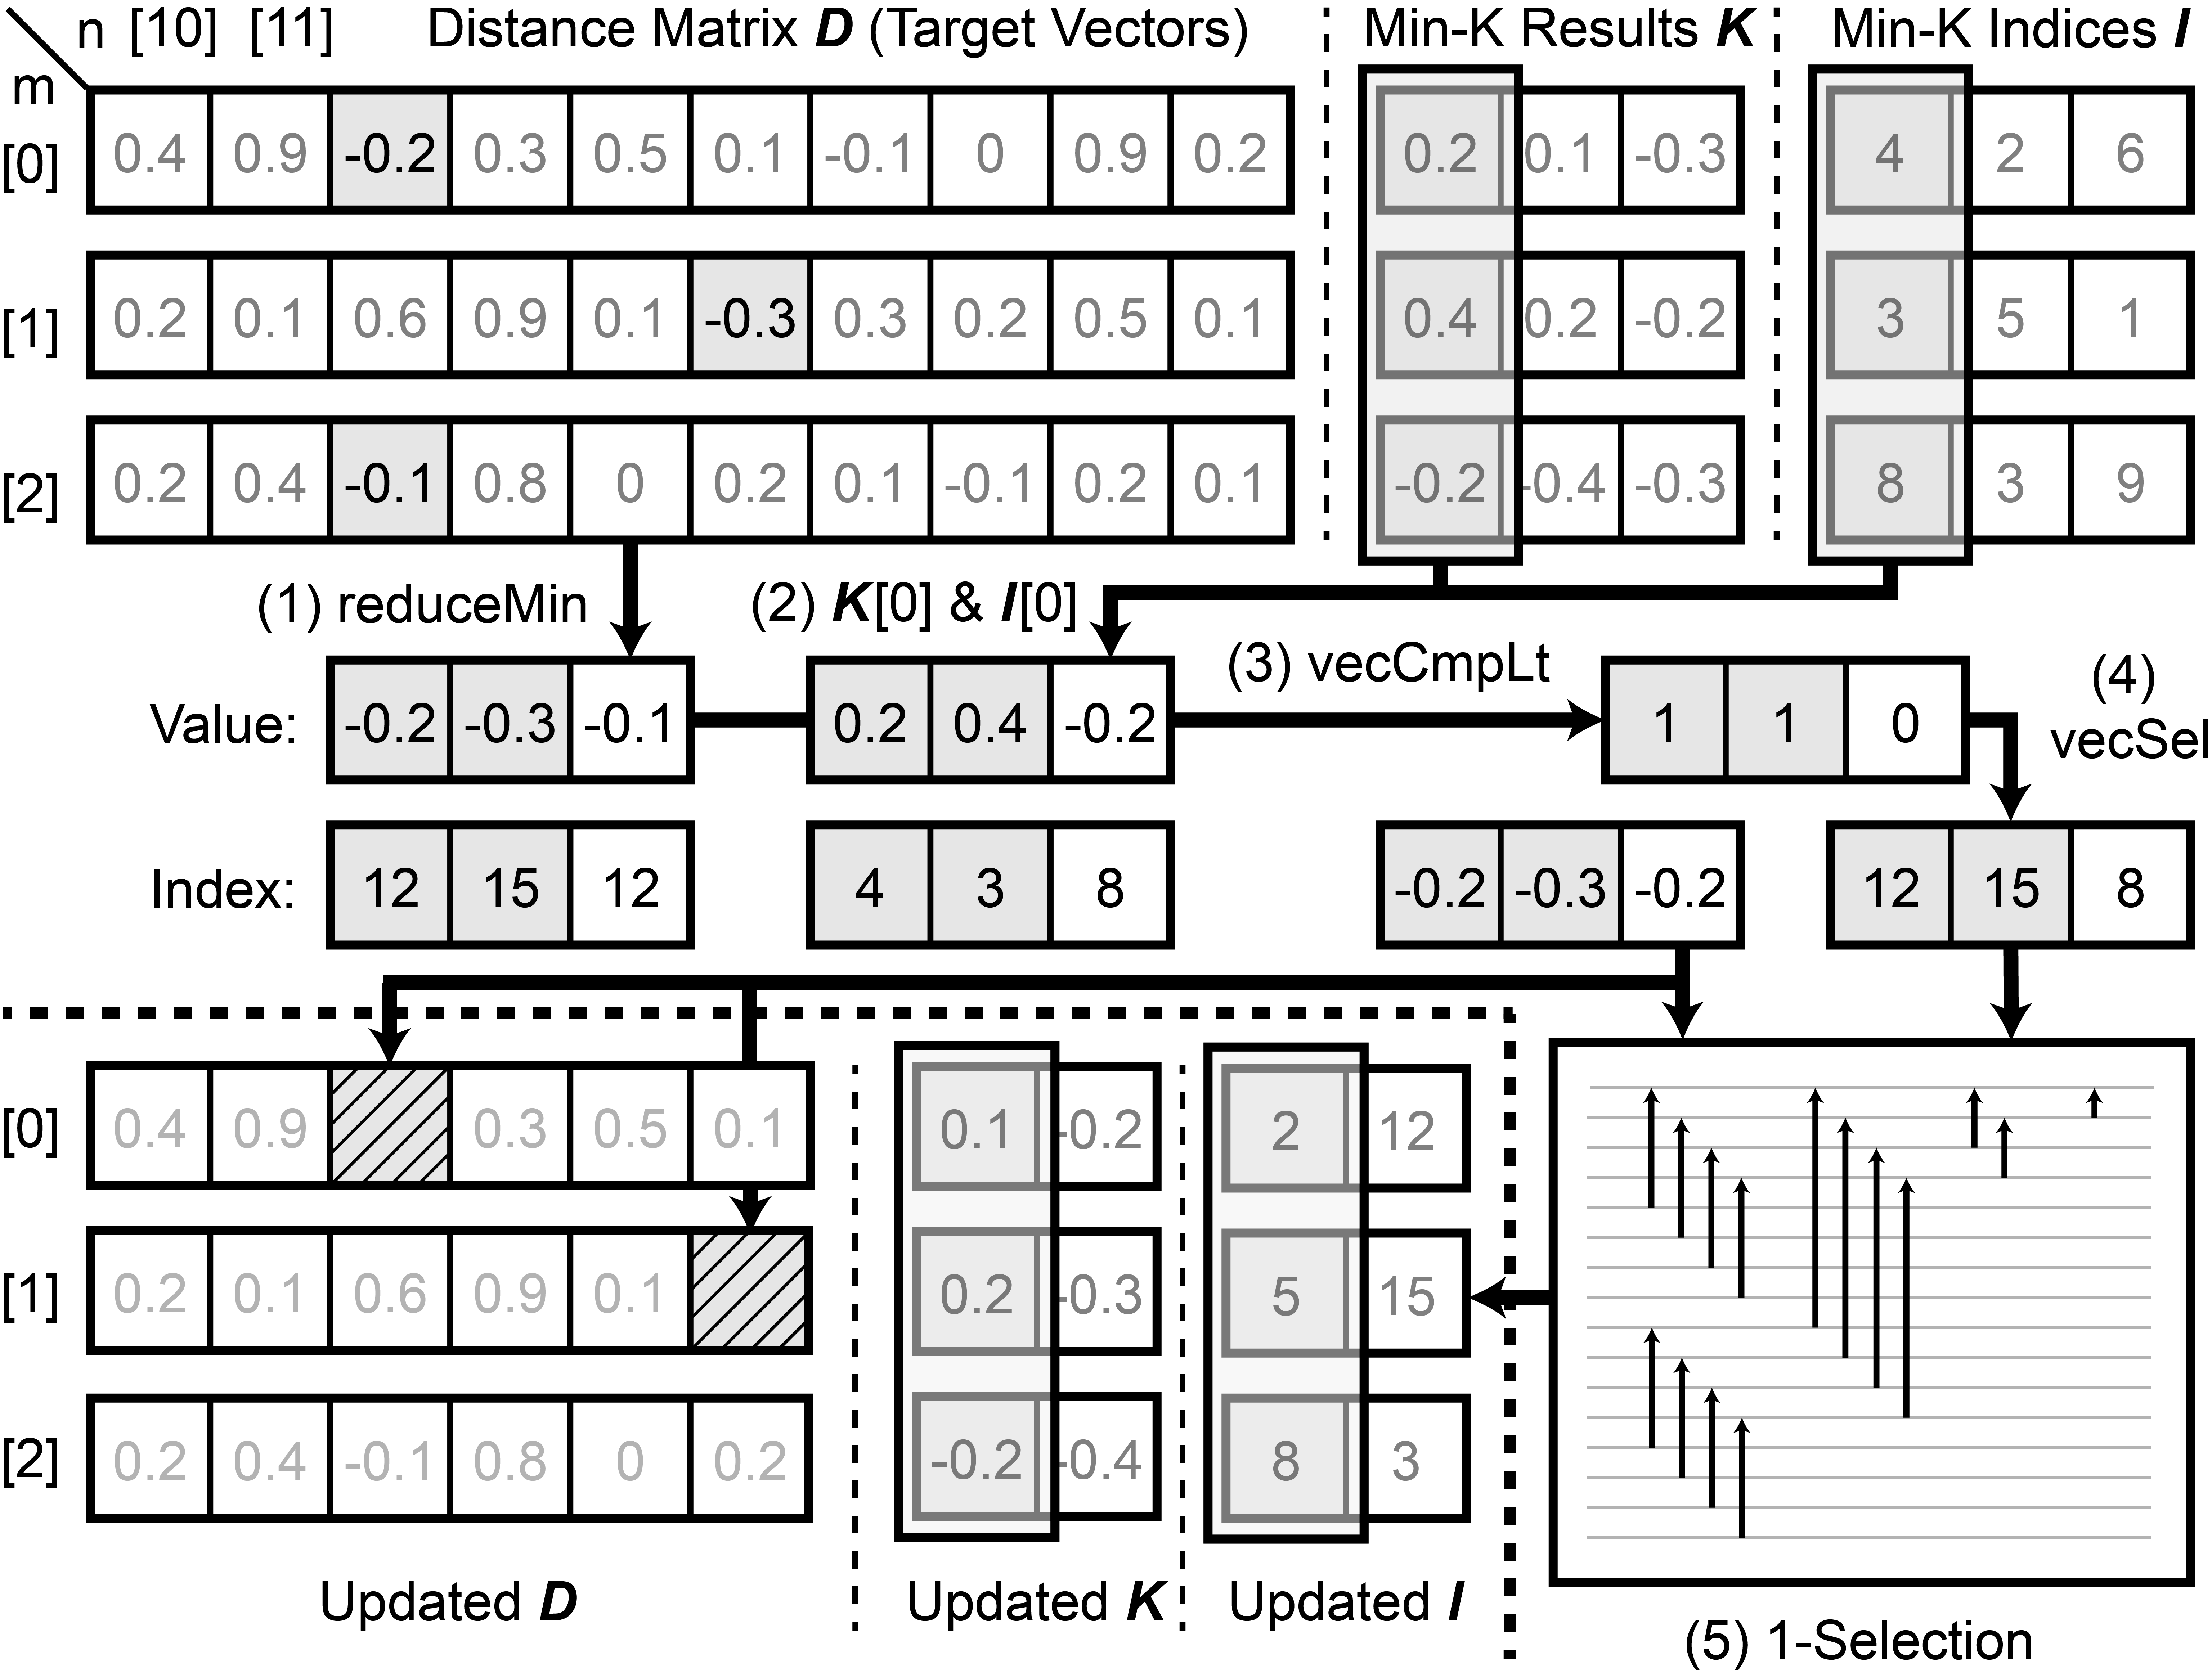
\includegraphics[scale=0.23]{figures/single_k_sel.png}}
    \caption{One step of the batch $(0, 1)$ of the \textit{k}-selection ($m_2 = 3, n_2 = 10$)}
    \label{fig:single_k_sel}
    \end{figure}

The main procedure of the algorithm is a \textit{k}-step loop. Fig. \ref{fig:single_k_sel} illustrates one \textit{step} example of the batch $(0, 1)$ of the \textit{k}-selection with the tiling shape of $m_2 = 3, n_2 = 10$, which process the data range of $m \in [0, 3), n \in [10, 20)$. The algorithm first find the minimum value $res_{min}$ with its index $idx_{min}$ in the target vector $\textbf{D}[ln]$. Then for $m$ target vectors, we compare whether $res_{min}$ is less than the first element of the min-\textit{k} results $\textbf{K}[0]$ in parallel. With the compared results, we update $\textbf{K}[0]$ and $\textbf{I}[0]$ accordingly. For the example in Fig. \ref{fig:single_k_sel}, $\textbf{K}[0][0]$ and $\textbf{K}[0][1]$ are updated since $-0.2 < 0.2$ and $-0.3 < 0.4$. The next step is the most significant step, where we maintain the min-\textit{k} results $\textbf{K}$ to ensure the first element is always the maximum element with the bitonic 1-selection. When $k=1$, the bitonic \textit{k}-selection is degenerated to a reduction but not only return the reduced value as \verb|reduceMax| does. Instead, it rearranges the vector and puts the top-$1$ value at the first element. Compared with directly invoking \verb|reduceMax|, the bitonic 1-selection avoids scalar dynamic addressing that locates the reduction results and variable assignments that update values for each target vector respectively. Instead, it calls $O(k)$ vectorized comparisons \& selections. On the other hand, the approach should not replace \verb|reduceMin| for the $n$-sized $\textbf{D}$, which would bring $O(n)$ vectorized comparisons \& selections as the direct bitonic-based approach does for the entire \textit{k}-selection. With the compared results, we also update value $res_{min}$ in the target vector with a large constant. 

For each test point, the time complexity of SelB-\textit{k}-NN \textit{k}-selection algorithm is $O(k + k^2 + nk)$, which consists of three parts, the scalar operation part, the vectorized comparison \& selection part, and other well-supported vectorized operations part. Although the overall time complexity seems to be higher than the heap-based \textit{k}-selection of $O(nlogk)$ and the bitonic-based \textit{k}-selection of $O(nlog^2k)$, our algorithm significantly reduces the scalar operations from $O(nlogk)$ to $O(k)$, and the vectorized comparisons \& selections from $O(nlog^2k)$ to $O(k^2)$, as annotated in Alg. \ref{alg:single_main}. SelB-\textit{k}-NN \textit{k}-selection algorithm prevents the less powerful operations of AI processors from growing with the scale of training dataset $n$. Existing works \cite{hassanat2014solving, abu2019effects} report that in \textit{k}-NN algorithm, a larger parameter \textit{k} does not contribute to higher accuracy. Therefore, we can safely assume that $n \gg k$, where our algorithm restrains the number of the scalar operations and vectorized comparisons \& selections for higher performance with acceptable accuracy.

The second feature of the algorithm is an early exit policy. For $m_2$ test points, we initialize an $m_2$-length vector $mask$ to '0's. The vector is updated each step based on the parallel comparison results by selecting the elements between $mask$ itself with '1's, as shown in line 10. All the values of those target vectors, whose minimum values are greater than the maximum values in their corresponding min-\textit{k} results, are greater than all the values in the min-\textit{k} results, as Eq. \ref{eq:main_equation} shows. 

\begin{equation}
    \label{eq:main_equation}
    \begin{aligned}
    \forall x \in \textbf{D}, res_{min} \le x &;\ 
        \forall y \in \textbf{K}, res_{max} \ge y \\
    res_{min} > res_{max} &\implies \forall x > \forall y
    \end{aligned}
\end{equation}

Therefore, once $res_{min} > res_{max}$, all the remaining values in the target vector are not the candidates of the min-\textit{k} results and can be rejected directly. Then the related element of $mask$ is updated to '1', and the algorithm skips the corresponding target vector, as shown in line 4. In the example of Fig. 3, the $\textbf{D}[2]$ is rejected in this step since $-0.1 > -0.2$. When the minimum value of $mask$ is not '0', which means all the elements are updated to '1', the algorithm ends in advance, as shown in line 11. For all batches after tiling the test dataset along \textit{m}-direction and the training dataset along \textit{n}-direction, each batch of SelB-\textit{k}-NN additionally receives the min-\textit{k} results from the last adjacent tile along \textit{n}-direction, as shown in \textbf{Input K} of Alg. \ref{alg:single_main}. The early exit policy can be activated by the last results and reduces most workloads during the execution. We will discuss the details of the workload reduction later in Sec. \ref{sec:tile}.

\section{Minimizing Hardware Support Requirements}

To minimize the hardware support as much as possible for portability of SelB-\textit{k}-NN, this section proposes two algorithms to replace the uncommon functions in DNNs with the most common functions on the AI processors \cite{cambricon, CANN, jax}.

\subsection{ReLU-Based Operations for VecCmp and VecSel \label{sec:relu}}

For the AI processors without \verb|vecCmp| and \verb|vecSel| hardware supports, we propose a novel \verb|ReLU|-based bitwise algorithm specifically for the AI processors. We do not involve bit-shifting or integer division to avoid extra requirements for hardware components on the AI processors.
    
\begin{algorithm}[tbp]
    \caption{Bitwise Ops for VecCmpLt and VecSel}
    \label{alg:bit_hack}
            
    \SetKwInOut{Input}{Input}
    \SetKwInOut{Output}{Output}
            
    \Input{
        compared vector \textbf{A, B} of FP16 numbers \\
        target vector \textbf{X, Y} of 16-bits numbers \\
    }
                
    \Output{
        result vector \textbf{R} from \textbf{X} and \textbf{Y}, based on the element-wise minimum between \textbf{A} and \textbf{B}
    }
    \BlankLine
    \#\# \textbf{VecCmpLt:} Computing \textit{mask} from \textbf{A, B} \\
    $\text{sub}_{1} \leftarrow \textbf{A} - \textbf{B}$ \\
    $\text{sub}_{2} \leftarrow (\text{sub}_{1} \  \& \  \vec{\textbf{0x8000}}) \mid \vec{\textbf{0x0001}}$ \\
    $\text{mask}_{1} \leftarrow \textbf{ReLU}(\text{sub}_{2})$ \\
    $\text{mask}_{2} \leftarrow \text{reinterpret} \  \text{mask}_{1} \  \text{as INT16 vector}$ \\
    $\text{mask} \leftarrow \text{mask}_{2} - \vec{\textbf{1}}$ \\
    
    \BlankLine
    \#\# \textbf{VecSel:} Computing \textbf{R} with \textit{mask} from \textbf{X, Y}\\
    $\textbf{R} \leftarrow \textbf{X} \ \&\ \text{mask}$ \\
    $\textbf{R} \leftarrow \textbf{R} \mid (\textbf{Y} \ \&\ \sim \text{mask})$ \\
\end{algorithm}
    
We show the algorithm in Alg. \ref{alg:bit_hack} for \verb|vecCmpLt| and \verb|vecSel|, which generates a mask based on the smaller elements of the two vectors and then selects values from the other two target vectors with the mask. For any vector \textbf{A} and \textbf{B}, Alg. \ref{alg:bit_hack} first computes the the vectorized subtraction results $sub_{1}$. Then it masks out the exponent and mantissa part (last 15 bits) of the FP16 number $sub_{1}$ and then sets the last bit to '1' by a bitwise inclusive OR operation. For the element where $A < B$, the $sub_{2}$ is 0x8001, while for $A > B$, the $sub_{2}$ is 0x0001. The essence and the most novel part of the algorithm is line 3, where it computes the comparison mask $mask_{1}$ with \verb|ReLU|, which is one of the most representative activation functions. The binary form of \verb|ReLU| function is shown below:

\begin{equation}
    \label{eq:relu}
    \textbf{ReLU}(t) = \left\{
    \begin{aligned}
        &\text{0b0xxx}  &t = \text{0b0xxx} \  &(t \ge 0) \\
        &\text{0b0000} &t = \text{0b1xxx} \  &(t \le 0) \\
    \end{aligned}
    \right.
\end{equation}
    
where 'x' is any bit ('0' or '1'). For both floating-point and integer numbers, whose most significant bit (the 1st bit) is the sign bit, \verb|ReLU| checks the sign bit and returns the result values according to its formula. Therefore, after line 3, the $mask_{1}$ for $A < B$ is set to 0x0000, while for $A > B$ it is set to 0x0001. Alg. \ref{alg:bit_hack} reinterprets $mask_{1}$ as INT16 number, which requires no instructions but only indicates that the following operation is integer operations. Then Alg. \ref{alg:bit_hack} subtracts INT16 number 1 from the result following the integer arithmetic rules. After that, the final comparison mask $mask$ for $A < B$ becomes 0xffff ($-1$ in INT16), while for $A > B$, it becomes 0x0000. To compute the mask of $A > B$ (vecCmpGt), swap the input $\textbf{A}$ and $\textbf{B}$ and the rest part remains the same. For the mask of $A = B$ (vecCmpEq), the $sub_{1}$ is modified to be computed by the formula below with other parts unchanged:

\begin{equation}
    sub_{1} \leftarrow (\textbf{A} - \textbf{B}) \mid (\textbf{B} - \textbf{A})
\end{equation}

With the comparison masks, Alg. \ref{alg:bit_hack} then selects the values from the target vector \textbf{X} and \textbf{Y}. Line 6 masks the values in \textbf{X} vector where $A > B$ with the corresponding mask of 0x0000, and keeps values where $A < B$ with the mask of 0xffff. Line 7 finishes the symmetric jobs and combines the two results with a bitwise inclusive OR operation.

The replaced \verb|vecCmpLt| and \verb|vecSel| involves only several efficient vectorized operations on the AI processors, including \verb|ReLU|. \verb|ReLU| is innately designed to contain a branch operation but wrapped by its original algorithm. Our algorithm widens \verb|ReLU| with its branch operation to general purposes. The algorithm contains no scalar operations and can achieve high performance on the AI processors.

\subsection{Indexing with Vectorized Operations}

While \verb|reduceMin| (\verb|reduceMax|) is irreplaceable in the deep learning applications, returning the corresponding indices is not necessary to be supported on the AI processors. To migrate the algorithm to the AI processors without vectorized hardware indexing supports, we propose an efficient algorithm for indexing on those AI processors shown as Alg. \ref{alg:indices_search}. The algorithm has one more vectorized operations than the \textit{k}-selection algorithm, \verb|vecDup|, which assigns a value to the whole vector and is also commonly used in the initialization of each layer.

\begin{algorithm}[tbp]
    \caption{Indexing w/ vectorized operations}
    \label{alg:indices_search}
        
    \SetKwInOut{Input}{Input}
    \SetKwInOut{Output}{Output}
        
    \Input{
        indexing vector \textbf{K} of size (n) \\
        indexing target value V
    }
            
    \Output{
        index of value V in vector \textbf{K}
    }
    \BlankLine
    
    $\text{idxMap} \leftarrow [0, 1, 2, \dots, (\text{n}-1)]$ \\
    $\text{vArray} \leftarrow [\text{V}, \text{V}, \text{V}, \dots, \text{V}]$ \\
    $\text{cmp} \leftarrow $ \textbf{vecCmpEq}$(\text{vArray}, \textbf{K})$  \\
    $\text{idxArray} \leftarrow $ \textbf{vecSel}$(\text{cmp}, \text{idxMap}, \vec{\textbf{0xfc00}})$ \\
    $\text{V} \leftarrow$ \textbf{reduceMax}$(\text{idxArray})$ \\
\end{algorithm}

The algorithm first assigns the target value $V$ to an $n$-sized array $vArray$ with \verb|vecDup|. Then it compares the $vArray$ with the indexing vector \textbf{K} to build a bitmask with \verb|vecCmpEq| for the position where $V$ locates. With the comparison mask $cmp$, we select the indices data between a prepared indices map $idxMap$ and an array full of 0xfc00 to build a result array $idxArray$. With \verb|reduceMax|, the algorithm finds the result index of indexing target value $V$. Since the indexing algorithm has no scalar operations, it would not be the bottleneck of the whole \textit{k}-selection algorithm.

One tricky part is the value 0xfc00. Most AI processors \cite{DBLP:journals/micro/ChoquetteGGSK21, DBLP:conf/isca/LiuDTHLXCC16, DBLP:conf/isca/JouppiYPPABBBBB17, DBLP:conf/hotchips/LiaoTXZ19} adopt FP16 as the computation data type to save the storage and improve the performance. Therefore, the vectorized operations usually fully support FP16 data on these AI processors but support INT16 data partially, e.g., subtraction we used in Sec. \ref{sec:relu}. For \verb|vecCmpEq| operations without INT16 data supports, since it does not rely on the numerical value of the data, we can directly cast the INT16 indices data to FP16 with no bit modifications. However, for \verb|reduceMax|, we need to ensure that the final index we find is numerically greater than others in FP16 format. Therefore, we select the value 0xfc00 as the initialized value, which is the negative infinity of FP16 and is less than all other 16-bit data in FP16 format. In this way, when we still cast our INT16 indices data to FP16 without any format conversions, \verb|reduceMax| still works no matter how the bits represent in FP16 format. One potential issue is that when multiple target values $V$ exist in the vector, we cannot ensure which index will be returned. However, it makes no trouble in our \textit{k}-selection algorithm. In addition, on the AI processors that support INT16 vectorized operations, the value 0xfc00 still works well. The value 0xfc00 is negative in INT16 format (-1023) and less than all possible indices.

\section{Optimal Tiling Shape Search \label{sec:tile}}

As illustrated in Fig. \ref{fig:tiling}, the parameters $(m_1, n_1)$ and $(m_2, n_2)$ determine the tiling (or batch) shapes of the distance computation and the \textit{k}-selection, which significantly influences the entire performance. This section discusses how we find the optimial tiling shapes with an optimization problem.

\subsection{\textit{K}-selection Workload Quantification \label{kSel}}

Along the $n$-direction, while each tile of the matrix multiplications has stable and equal workloads, the workload of each tile in SelB-\textit{k}-NN \textit{k}-selection varies based on its assigned datasets and last min-\textit{k} results. During the runtime of the algorithm, the early exit policy of the \textit{k}-selection is continually activated by the last adjacent tile's results. It dynamically rejects the for-loop steps of the \textit{k}-selection as shown in Alg. \ref{alg:single_main}, identified as the primary workloads. Intuitively, the later tiles always have fewer workloads. To accurately model the algorithm performance to an optimization problem, we present an analysis to quantify the \textit{k}-selection workload of the tile $t$.

Let us assume that for a specific test data $m$, the distance computation results of all training data $D$ obey some random distribution $\mathcal{F}(X)$. Therefore, after the computation of tile $t$ during the execution, the distance computation results that have been computed $D_{1 \to t}$ and are computed just at the computation of tile $t$, $D_{t}$, also obey the distribution $\mathcal{F}(X)$.

\begin{equation}
    \begin{aligned}
        D \sim \mathcal{F}(X) \implies D_{1 \to t}, D_{t} \sim \mathcal{F}(X)  
    \end{aligned}
\end{equation}


Then let us consider that after the tile $t$, $x^{\prime}_{1 \to t}$ is the \textit{k}-th minimum value of $D_{1 \to t}$, which is also the maximum value of the \textit{k}-min results. We can compute the cumulative distribution function (CDF) of the distribution $\mathcal{F}_{X}(x^{\prime}_{1 \to t})$ as follows:

\begin{equation}
    \mathcal{F}_{X}(x^{\prime}_{1 \to t}) = P(X \le x^{\prime}_{1 \to t}) = \frac{k}{nt}
\end{equation}

where $n$ is the number of distance results of each tile (also the number of \textit{k}-selection inputs). The CDF computes the probability of randomly selecting a value from $D_{1 \to t}$, which is one of the \textit{k}-min results. Let us call that for the tile $t$, the values, which belong to the distance results $D_{t}$ and are going to replace another value in the current \textit{k}-min results, are \textit{updating} values. Then for the tile $t$, when one value $x$ is updating at this stage, it means that $x \le x^{\prime}_{1 \to t}$. Therefore, for the tile $t$ of size $n$, the expected number of the updating value can be computed by the CDF as follows:

\begin{equation}
    E_{t}(X \le x^{\prime}_{1 \to t}) = n \mathcal{F}_{X}(x^{\prime}_{1 \to t}) = \frac{k}{t}
\end{equation}


Since each for-loop \textit{step} of SelB-\textit{k}-NN \textit{k}-selection in Alg. \ref{alg:single_main} updates one value, the expected \textit{updating} value is also the expected \textit{step} number for tile $t$. Hence, for tile $t$, the workload of the \textit{k}-selection phase is quantified to $k / t$ theoretically.

\subsection{Execution Time Optimization Problem Formulation}

For the entire test dataset of $(M \times d)$ and the training dataset of $(d \times N)$, let us consider the tiling shape $(m_{1}, n_{1})$ for the distance computation phase and $(m_{2}, n_{2})$ for the \textit{k}-selection phase. As we discussed in Sec. \ref{sec:tiling}, since the tiling shapes of $k$-selection are restricted by those of distance computation, we have $m_{2} \le m_{1}, n_{2} \le n_{1}$. Our goal is to minimize the overall execution time by a space exploration of the four tiling shapes $(m_{1}, n_{1})$ and $(m_{2}, n_{2})$. Formally, we formulate the following optimization problem.

\begin{equation}
    \label{eq:optimized}
    \begin{aligned}
        min\quad  &T_{mm} + T_{kSel} \\
        s.t.\quad &T_{mm} = \frac{MN}{m_{1}n_{1}} f(m_{1}, n_{1}) \\
                  &T_{kSel} = \frac{M}{m_{2}} \sum_{t=1}^{\frac{N}{n_{2}}}(\frac{k}{t}g(m_{2}, n_{2}) + g_{0}(m_{2}, n_{2})) \\
                  &d(m_1 + n_1) + m_2(n_2 + k) < Size_{mem} \\
                  &m_{2} \le m_{1}, n_{2} \le n_{1} \quad \quad (*)
    \end{aligned}
\end{equation}

where $f(m_{1}, n_{1})$ is the profiled execution time of the matrix multiplication with the tiling shape $(m_{1}, n_{1})$, $g(m_{2}, n_{2})$ is the execution time of a \textit{step} in \textit{k}-selection (line 3 to 15 in Alg. \ref{alg:single_main}) with the tiling shape $(m_{2}, n_{2})$ with constant cost $g_{0}(m_{2}, n_{2})$, $Size_{mem}$ is the size the on-core memory.

\subsection{Search Space Pruning}

The search space size of the optimization problem in Eq. \ref{eq:optimized} is $O(m^2n^2)$, which can be very large and time-consuming to search exhaustively. This subsection adds one more constraint to prune its search space to $O(m^2n)$.

For the optimized solutions, the search procedure contains a four-layer loop to search the parameters. It firsts select a set of $(m_{1}, n_{1})$ in the outer loops, and then traverse all $(m_{2}, n_{2})$ in the inner loops with the constraint $(*)$. At the innermost loop for $n_{2}$ search, while $(m_{1}, n_{1}, m_{2})$ are selected, let we consider $pn_{2} = n_{1}$, where $p \ge 1$. Then we have:

\begin{equation}
    \begin{aligned}
        T_{kSel}(m_{2}, n_{2}) = 
            \frac{M}{m_{2}} \sum_{t=1}^{\frac{pN}{n_{1}}}(\frac{k}{t}g(m_{2}, \frac{n_{1}}{p}) + g_{0}(m_{2}, \frac{n_{1}}{p}))
    \end{aligned}
\end{equation}

If $T_{kSel}(m_{2}, n_{2}) > T_{kSel}(m_{2}, n_{1})$ always holds, it means that for any $p > 1$ (or for any $n_{2} < n_{1}$), the execution time is longer compared with the exeuction time when $n_{2} = n_{1}$. Therefore, let us consider:


\begin{equation}
    \begin{aligned}
        T_{kSel}(m_{2}, n_{2}) &> T_{kSel}(m_{2}, n_{1}) \\
        \sum_{t=1}^{\frac{pN}{n_{1}}}(\frac{k}{t}g(\frac{n_{1}}{p}) + g_{0}(\frac{n_{1}}{p})) &> \sum_{t=1}^{\frac{N}{n_{1}}}(\frac{k}{t}g(n_{1}) + g_{0}(n_{1}))
    \end{aligned}
\end{equation}

where we simplify $g(m_{2}, n)$ to $g(n)$. Then we have:


\begin{equation}
    \label{eq:ineq}
    \begin{aligned}
        \frac{N}{n_{1}}(pg_{0}(\frac{n_{1}}{p}) - g_{0}(n_{1})) + k &(\sum_{t=1}^{\frac{pN}{n_{1}}}\frac{g(\frac{n_{1}}{p})}{t} - \sum_{t=1}^{\frac{N}{n_{1}}}\frac{g(n_{1})}{t}) > 0
    \end{aligned}
\end{equation}

Notice that:


\begin{equation}
    \begin{aligned}
        k (\sum_{t=1}^{\frac{pN}{n_{1}}}\frac{g(\frac{n_{1}}{p})}{t} - \sum_{t=1}^{\frac{N}{n_{1}}}\frac{g(n_{1})}{t}) > - k \sum_{t=1}^{\frac{N}{n_{1}}}\frac{g(n_{1})}{t} > - \frac{kN}{n_{1}} g(n_{1})
    \end{aligned}
\end{equation}

Then Eq. \ref{eq:ineq} is converted to:


\begin{equation}
    \label{eq:last}
    \begin{aligned}
        pg_{0}(\frac{n_{1}}{p}) - (&g_{0}(n_{1}) + kg(n_{1})) > 0
    \end{aligned}
\end{equation}

Since the inequality above does not involve input $N$, after profiling the execution time (e.g., $g(n_{1})$) on the AI processors, the search space can be reduced in advance in the preprocessing stage. For a set of selected $(m_{1}, n_{1}, m_{2})$, when $n_{2}$ satisfies the inequality above, the search for $n_{2}$ should be pruned directly as $n_{1} = n_{2}$. In addition, the inequality can be explained qualitatively. It suggests that for \textit{k}-selection with the tiling shape $n_{1}$, we further divide $n_{1}$ into $p$ smaller tiling shapes $n_{2}$. If the constant cost of the $p$ smaller tiling shapes' execution time ($pg_{0}(\frac{n_{1}}{p})$) is larger than the maximum execution time of the original tiling shape $n_{1}$ ($g_{0}(n_{1}) + kg(n_{1})$), the division of the $p$ tiles is ineffective.

\begin{figure}[htbp]
    \begin{adjustbox}{addcode={
        \begin{minipage}{\width}}{
            \caption{The single execution results of several \textit{k}-NN algorithm kernels}
            \label{fig:single}
        \end{minipage}},rotate=90,center}
        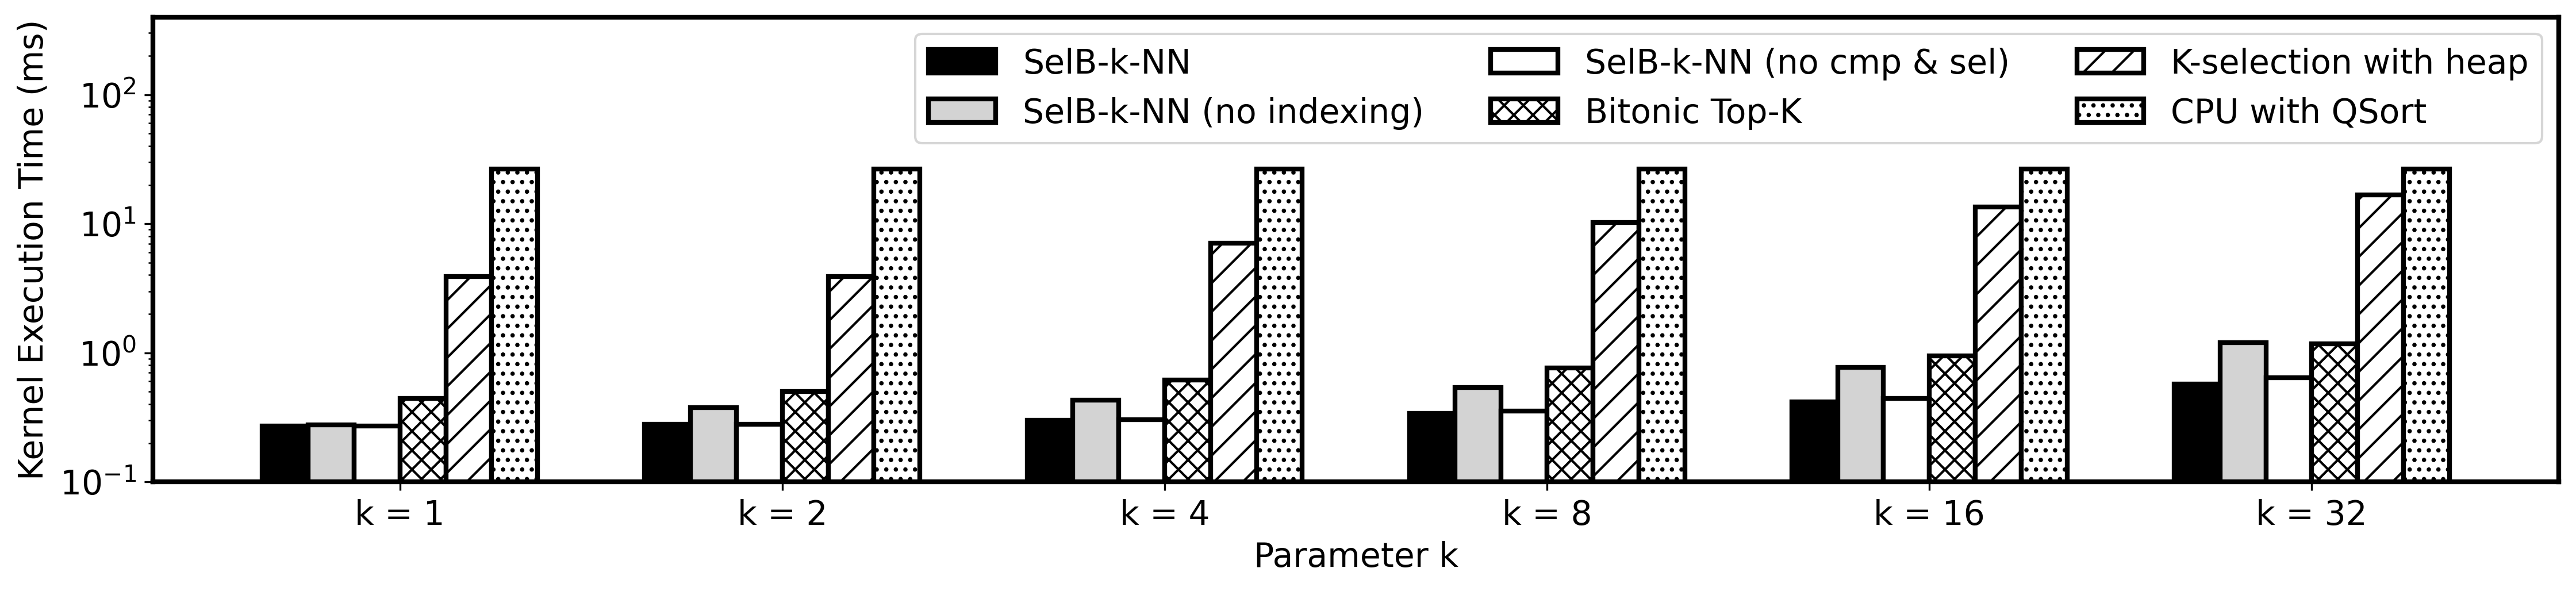
\includegraphics[scale=0.5]{figures/single_core.png}
    \end{adjustbox}
\end{figure}

\section{Evaluation}

We implement SelB-\textit{k}-NN algorithm on Huawei Ascend AI processors based on DaVinci \cite{DBLP:conf/hotchips/LiaoTXZ19} architecture for evaluation. The essence of the Ascend AI processors is DaVinci AI Cores, which provide 4 TFLOPS (FP16) or 8 TOPS (INT8) computation power per core. In addition to the hardware, Huawei also introduced a full-stack programming framework called AI Heterogeneous Compute Architecture (CANN) \cite{CANN}. We program all experiments with Tensor Boost Engine (TBE) and Tensor Iterator Kernel (TIK) for DaVinci kernel programming on CANN. For the matrix multiplication phase, we directly use the official native functions in CANN libraries. The detailed hardware model we used is the Huawei Ascend 310 processor (two DaVinci AI Cores installed) with 2 vCPUs of Intel Cascade Lake 6278 2.6GHz. All experiment results are wall-clock execution period from the start of the distance computation kernel to the end of the \textit{k}-selection kernel (or the end of \textit{k}-selection computation in the CPU approaches). For the evaluation dataset, since SelB-\textit{k}-NN is insensitive to the data distribution, we build randomly generated synthetic datasets. The data points are 128-dimensional with the value of each dimension in the range of $[-1, 1]$ on normal distribution.

\subsection{Single Execution of SelB-k-NN}

We compare SelB-\textit{k}-NN with the bitonic \textit{k}-selection approach, heap-based approach on the AI processors, and host CPU C++ STL quick sort approach. The distance computations of all approaches are accelerated by the Matrix MACs. We offer the implementation results without hardware indexing and \verb|vecCmp| \& \verb|vecSel| supports for the SelB-\textit{k}-NN algorithm. Fig. \ref{fig:single} shows the results of the test cases where the size of the test dataset is $(32 \times 128)$, and the size of the training dataset is $(128 \times 4096)$. We analyze the performance changes with the variation of the parameter \textit{k} of \textit{k}-NN.

\subsubsection{Overall Performance}

Generally, SelB-\textit{k}-NN algorithm reports incredible accelerations. It achieves an average acceleration of 2.01$\times$ compared with the bitonic approach, 23.93$\times$ compared with the heap approach, and 78.52$\times$ compared with the CPU quicksort implementation. With the increment of the parameter \textit{k}, except for the CPU quicksort, which has a constant workload, the execution time of the other implementations increases accordingly. The execution time of SelB-\textit{k}-NN when $k = 32$ grows to 1.55$\times$ compared with that when $k = 1$, while the bitonic approach increases to 2.13$\times$ and the heap approach rises to 3.45$\times$. Although the overall time complexity of SelB-\textit{k}-NN is $O(k + k^2 + nk)$, which theoretically increases faster than the other approaches with that of $O(nlog^2k)$ and $O(nlogk)$, the practical experiments report the opposite results. The abnormal behavior is mainly because of the inefficient performance of the weakly-supported scalar operations, vectorized comparisons \& selections on the AI processors, as we discussed. Time complexity assumes that all operations are equal, which is false on the AI processors. It evidences that the design principle of our SelB-\textit{k}-NN algorithm, to reduce the two operations as more as possible, meets the special hardware requirements of the AI processors. For the implementation without hardware indexing supports, the results show that the software indexing methods extend the execution time of the SelB-\textit{k}-NN algorithm to 1.56$\times$ averagely. For the implementation without hardware \verb|vecCmp| and \verb|vecSel| supports, our algorithm reports similar results with an average number of 1.04$\times$. At least in SelB-\textit{k}-NN, our software algorithm suffers a slight performance loss, which still achieves high efficiency on the AI processors.

\subsubsection{\textit{K}-Selection Early Exit \label{early}}

\begin{figure}[tbp]
    \centering{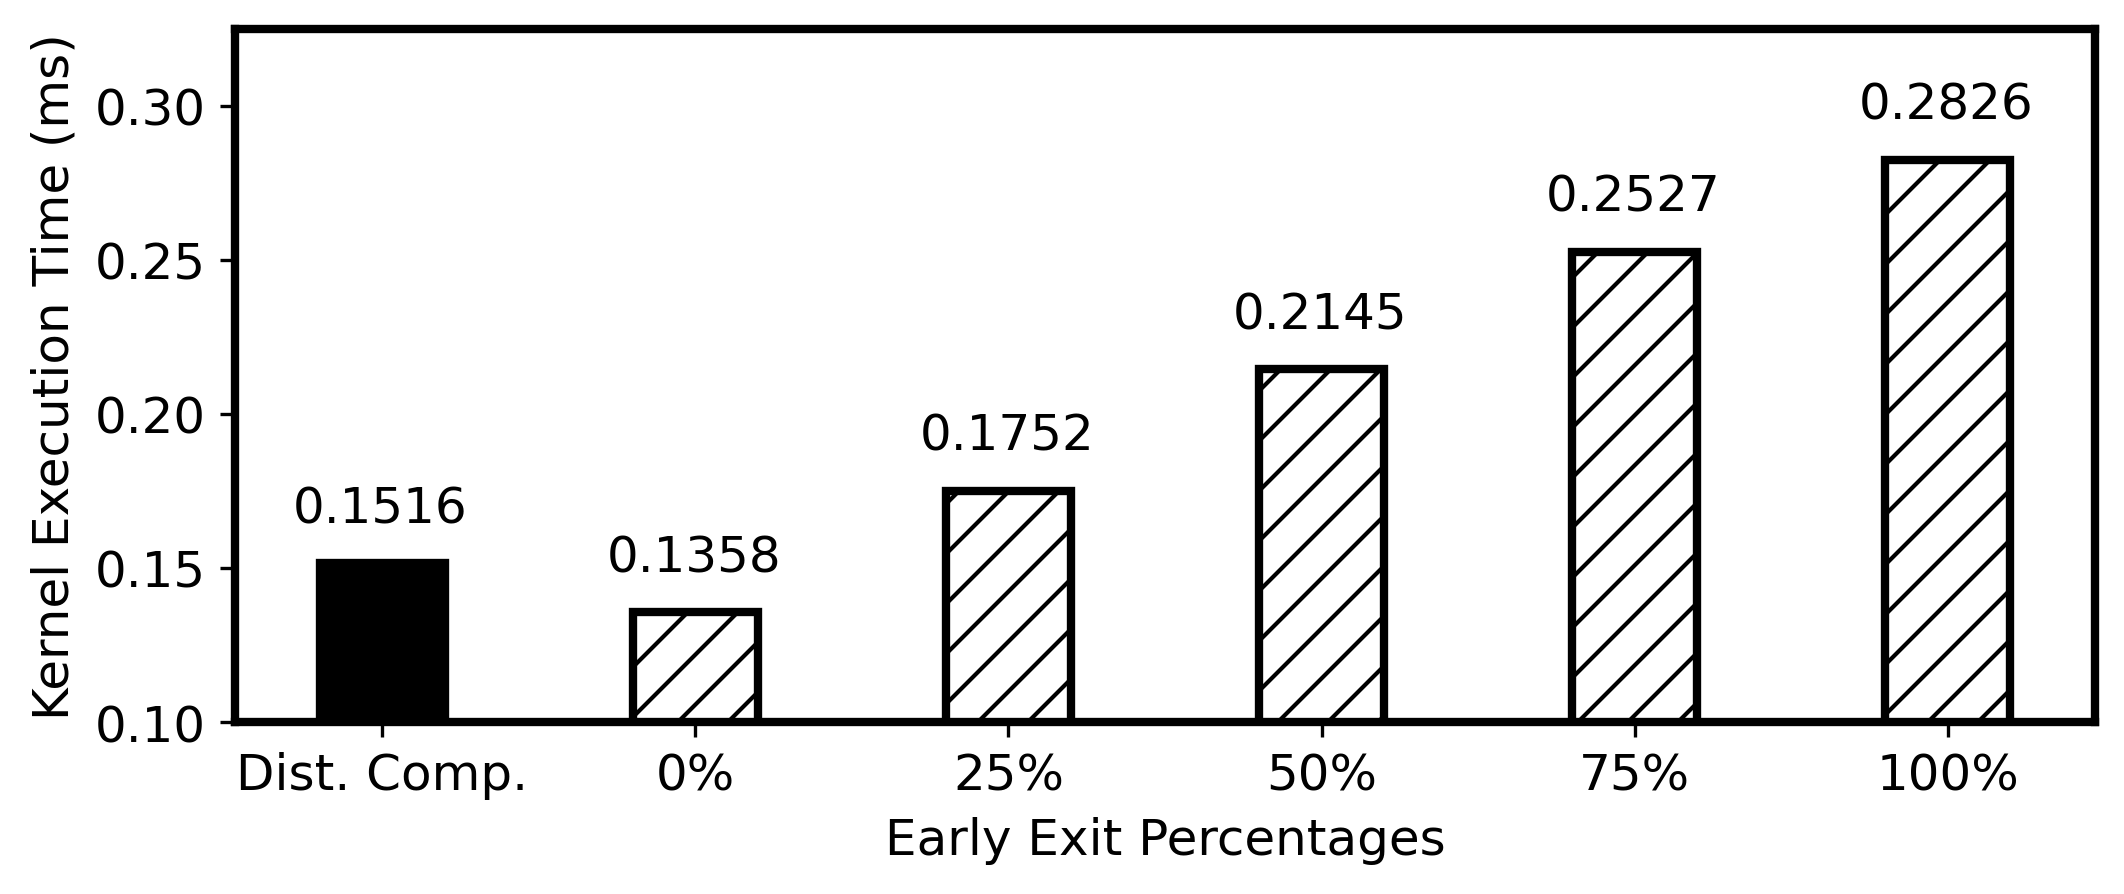
\includegraphics[scale=0.6]{figures/early_exit.png}}
    \caption{The \textit{k}-selection results with different early exit percentages}
    \label{fig:early_exit}
    \end{figure}

\begin{figure}[htbp]
    \begin{adjustbox}{addcode={
        \begin{minipage}{\width}}{
            \caption{The accelerations of the overall best best tiling shapes (MM + kSel) compared with the individual best tiling shapes (MM \& kSel)}
            \label{fig:final}
        \end{minipage}},rotate=90,center}
        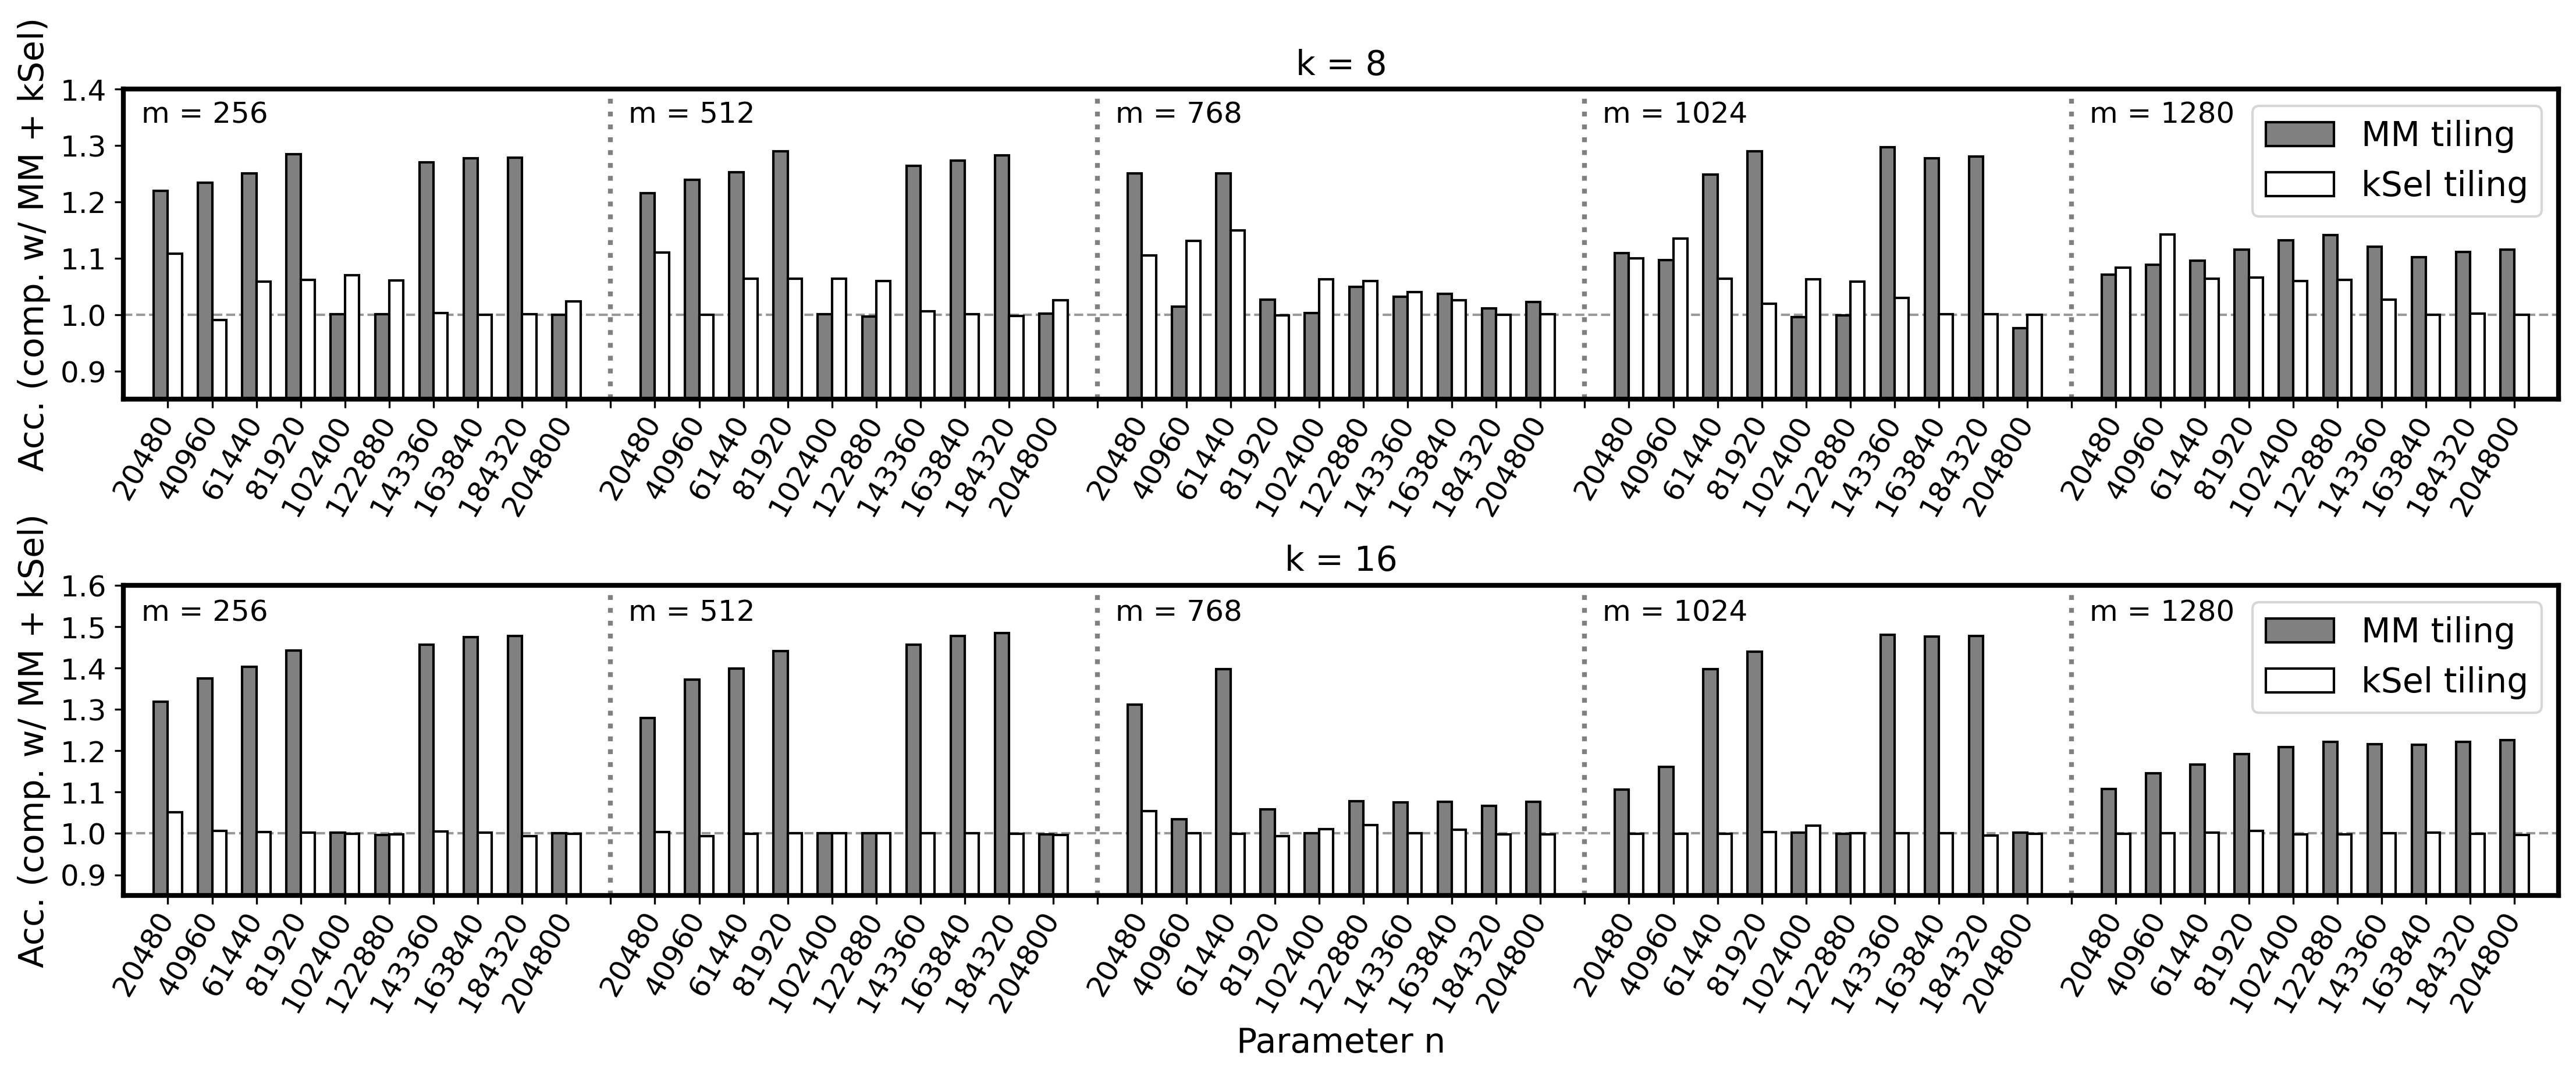
\includegraphics[scale=0.5]{figures/final_data.png}
    \end{adjustbox}
\end{figure}

By modifying the input datasets and the initial \textit{k}-min values, the number of updating values can be controlled intentionally. Therefore, we practically control and evaluate the execution time reduced by the early exit policy. Fig. \ref{fig:early_exit} illustrates the execution results for the case when $k = 16$ with the size of test dataset $(32 \times 128)$ and training dataset $(128 \times 4096)$. The early exit percentage represents the percentages of the workloads that have been done when the algorithm exits. We also add the execution time of the distance computation kernel to compute the exact proportion of the whole algorithm execution time being reduced.

The results report a linear growth of the \textit{k}-selection algorithm with the increment of the workloads. The \textit{k}-selection execution time of the case with all workloads is 2.08$\times$ than that with no workloads. For the whole algorithm execution time with the distance computation, the acceleration is 1.51$\times$. The results show that our early exit policy works well and significantly reduces the workload. In addition, even though there is no computation workload assigned to the kernel, the \textit{k}-selection algorithm still takes 0.1516 ms. The results show that the simple but slow scalar conditional branch operations take 48.22\% of the \textit{k}-selection kernel, which further shows the low performance of the scalar units on the AI processors.

\subsection{Mini-batch Execution of SelB-\textit{k}-NN}

\subsubsection{\textit{K}-selection Workload Quantification}

\begin{figure}[tbp]
    \centering{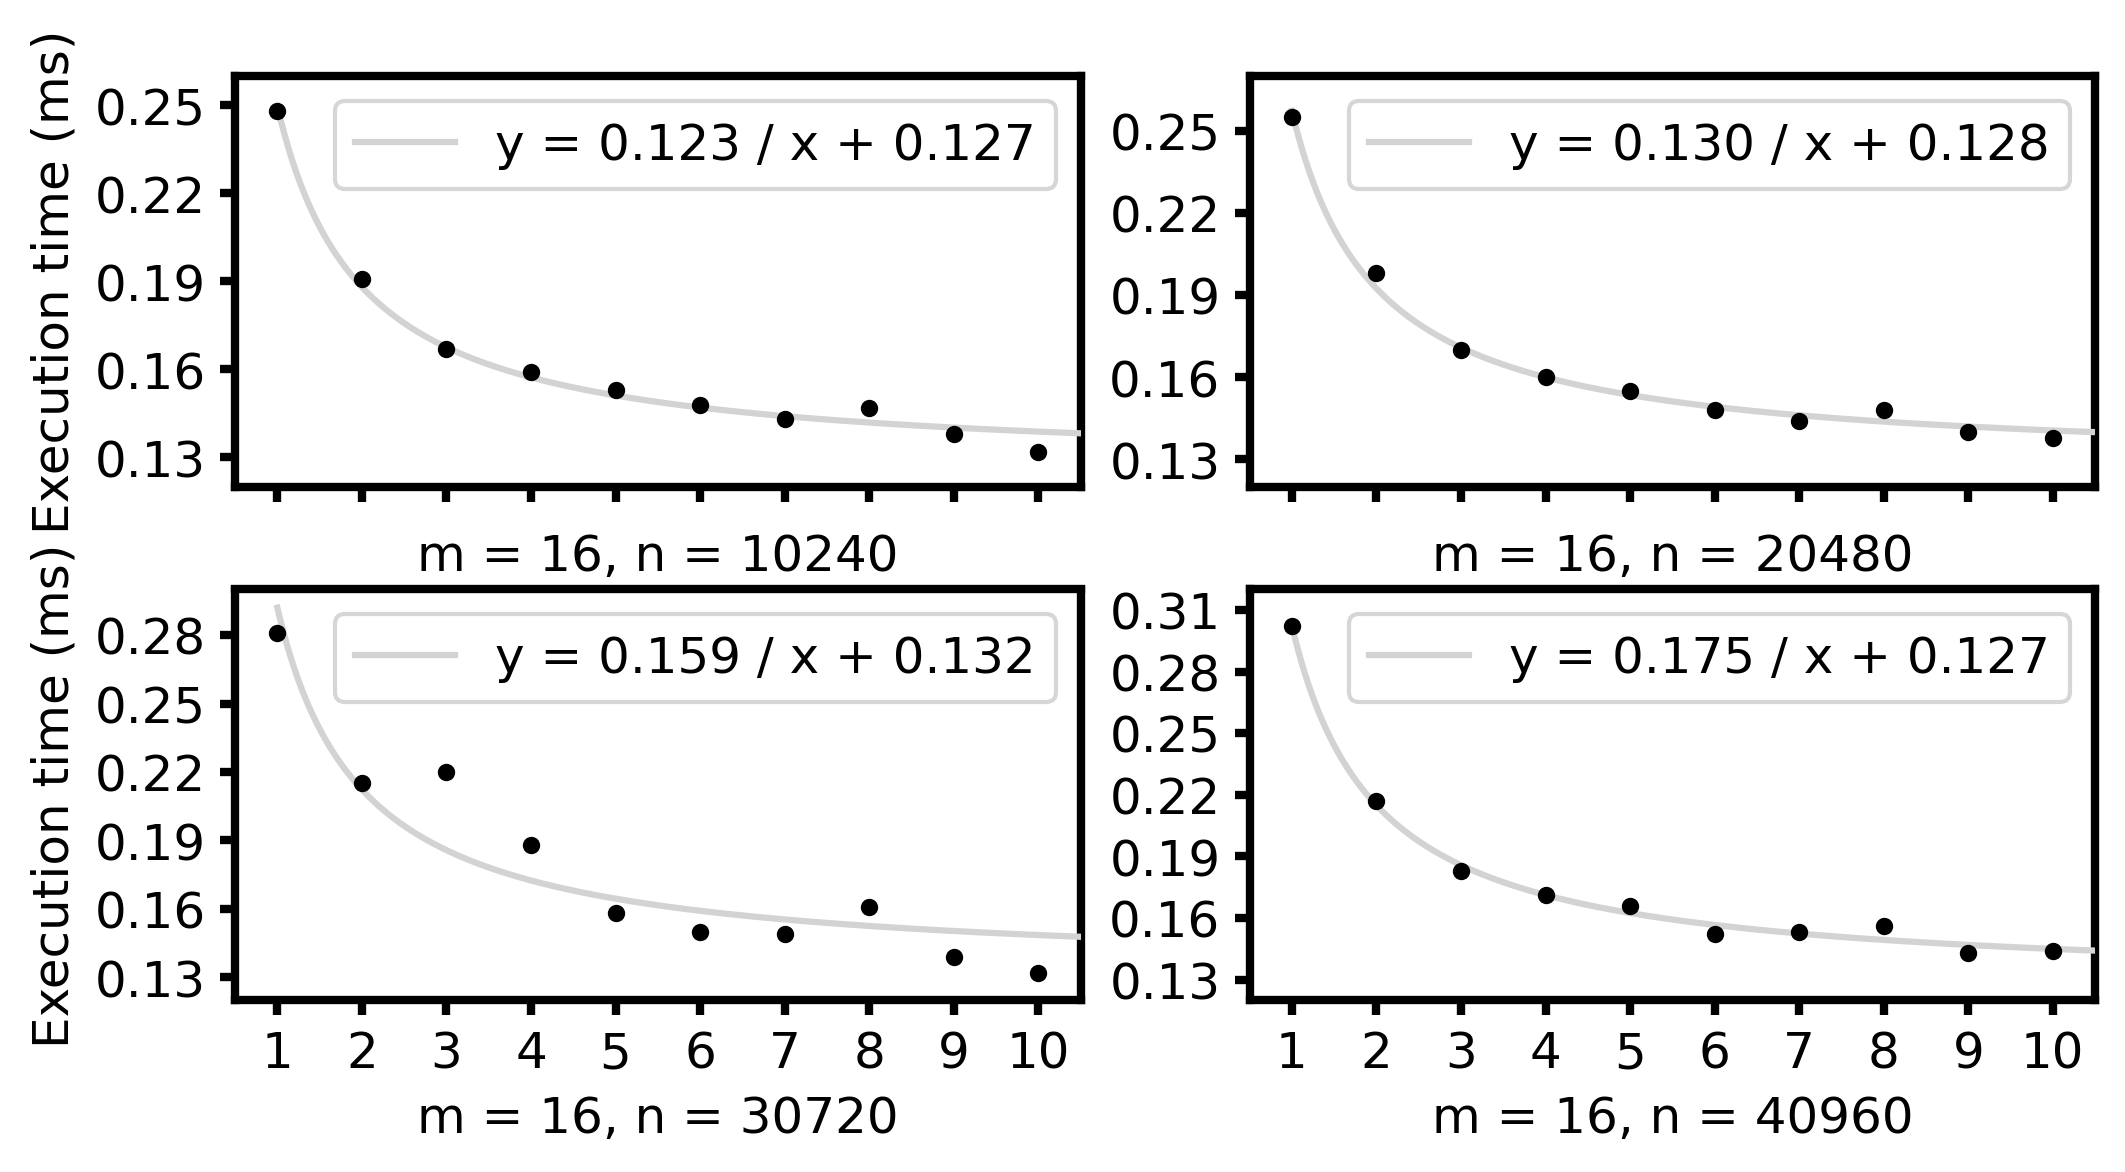
\includegraphics[scale=0.62]{figures/verified.png}}
    \caption{The \textit{k}-selection execution time of each tile and the fitting curves}
    \label{fig:verified}
    \end{figure}

We evaluate the execution time of sequential $k$-selection tiles after tiling, where each tile receives the min-$k$ results from the last adjacent tile to reduce its workloads. Fig. \ref{fig:verified} shows the evaluation results for four examples. The entire training dataset is divided into ten tiles along the $n$-direction. Each point in the figures represents the $k$-selection execution time of the \textit{t}-th tile.

For all four examples, the execution time decreases in an inverse proportion, as discussed in Sec. \ref{kSel}. The curves in the figures are fitted by the non-linear least squares method with an average coefficient of determination, $R^{2} = 0.97$. With the increment of $n$, the execution time of each \textit{t}-th tile increases plus a fixed constant cost of about 0.13 ms. For the example of $m = 16, n = 40960$, a tile is the single execution we shown in Sec. \ref{early}. Compared with the early exit results in Fig. \ref{fig:early_exit}, the workload being executed on each tile is apparent to be looked up, which also follows the inverse proportion. The curves and the workload variations evidence the correctness of our $k$-selection qualification.

\subsubsection{Mini-batch SelB-\textit{k}-NN Performance}

\begin{figure}[tbp]
    \centering{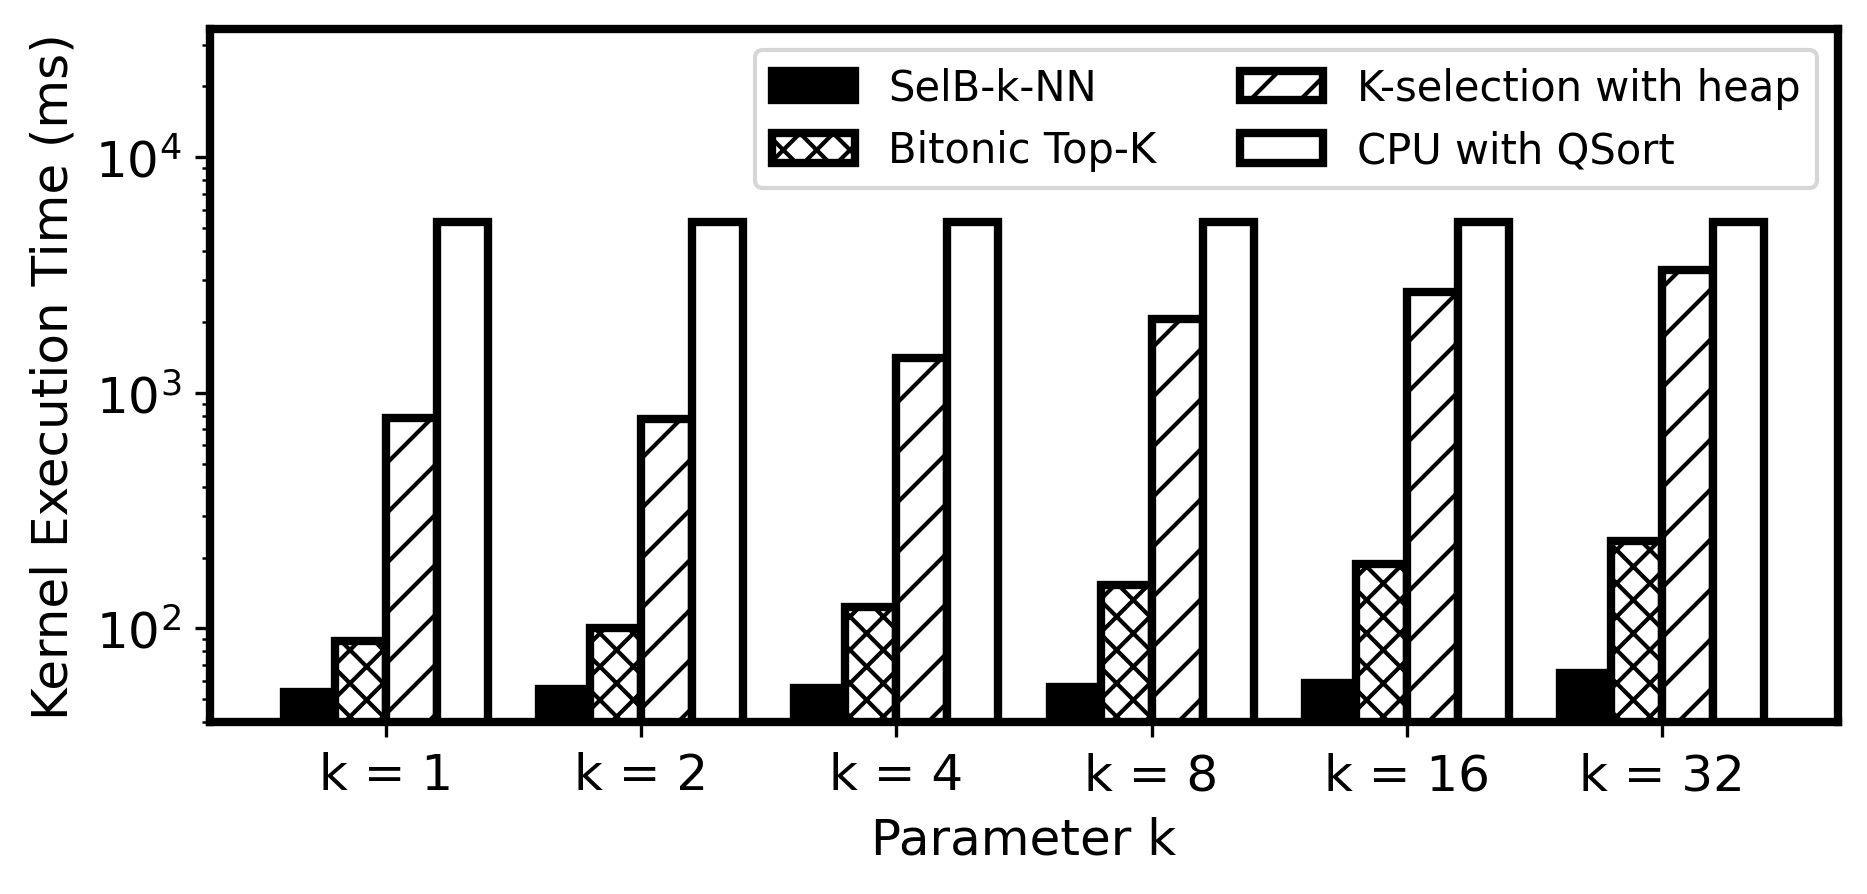
\includegraphics[scale=0.62]{figures/multi_results.png}}
    \caption{The \textit{k}-selection execution time of each tile and the fitting curves}
    \label{fig:multi_results}
    \end{figure}

We compare the performance of mini-batch SelB-\textit{k}-NN with other approaches with a larger dataset, where the test dataset is $(1280 \times 128)$ and the training dataset is $(128 \times 204800)$. The tiling shape we choose for SelB-\textit{k}-NN is $(16 \times 128)$ and $(128 \times 4096)$. 

Fig. \ref{fig:multi_results} shows the results for the comparison with different \textit{k}-values. Generally, compared with the single execution results, mini-batch SelB-\textit{k}-NN achieves higher accelerations. It reports an average speedup of 2.53$\times$ compared with the bitonic approaches, 31.24$\times$ with the heap approaches, and 92.75$\times$ with the CPU quicksort implementations. Meanwhile, with the increment of the \textit{k}-value, we observe the accelerations of SelB-\textit{k}-NN compared with other algorithms also grow significantly. The main reason for the higher accelerations is the early exit policy in SelB-\textit{k}-NN, which skipped most of the mini-batches in the large training dataset. 

\subsubsection{Tiling Shapes Results}

We evaluate the performance of SelB-\textit{k}-NN with different tiling shapes. We first profile the execution time of the matrix multiplication, $f(m_1, n_1)$, and that of the $k$-selection, $g(m_2, n_2)$ and $g_{0}(m_2, n_2)$. Then with the collected performance data, we solve the optimization problem in Eq. \ref{eq:optimized} for the optimal tiling shape $(m_1, n_1, m_2, n_2)$. In addition, we also solve the individual optimization problem of the matrix multiplication $(m_1, n_1)$ and \textit{k}-selection $(m_2, n_2)$ to apply them to the both phases for comparisons.

Fig. \ref{fig:final} illustrates the acceleration rates of the optimal tiling shapes (MM + kSel) compared with the other two tiling shapes (MM \& kSel) for the cases $k = 8$ and $k = 16$. Since the execution time of the CANN native matrix multiplication does not increase linearly with the expansion of the tiling shapes, the acceleration rates vary irregularly. Compared with the matrix multiplication tiling shapes, the optimal tiling shapes achieve an acceleration of 1.29$\times$ when $k = 8$ and 1.48$\times$ when $k = 16$. The acceleration is 1.14$\times$ when $k = 8$ and 1.05$\times$ when $k = 16$ compared with the \textit{k}-selection tiling shapes. The figure shows that the matrix multiplication tiling shapes significantly lower the performance in most cases. In contrast, the performance with the \textit{k}-selection tiling shapes is closer to that with the optimal tiling shapes. Moreover, the optimal tiling shape acceleration compared with the best matrix multiplication tiling shapes when $k = 16$ is larger than $k = 8$. The results are opposite for the acceleration compared with the best \textit{k}-selection tiling shapes. It is because when $k = 16$, the matrix multiplication occupies more proportions of the algorithm execution time. The whole execution is mainly determined by the \textit{k}-selection phase, which performs poorly with the matrix multiplication tiling shapes. Although the matrix multiplication also has a performance loss with the \textit{k}-selection tiling shapes, the execution time increment is far less than the decrement by the $k$-selection phase. For the case when $k = 8$, the reasons are symmetric. On the other hand, in some cases, the two tiling shapes both cause a worse performance than the performance with overall tiling shapes, where two phases have similar influences on the whole execution time.

In addition, with our pruning method, for the case when $k = 8$, 72.80\% of the optimization problem's search space is reduced; for $k = 16$, 55.23\% of the space is reduced. The percentage of the pruned domain is related to parameter $k$, which determines the proportion of the constant cost to the execution time related to the workloads of the $k$-selection.

\section{Conclusion}

This chapter introduced SelB-\textit{k}-NN, which is a novel \textit{k}-NN algorithm specifically designed for the AI processors. Based on the fact that the scalar operations, vectorized comparisons \& selections perform unexpectedly poorly on the AI processors, the main idea of SelB-\textit{k}-NN is to decrease the two operations as much as possible by combining the selection sort and bitonic $k$-selection. Since the AI processors produced by different manufacturers have various designs, we propose two algorithms to reduce hardware support requirements to the most critical operations of deep learning. Especially, the involvement of \verb|ReLU| in the bitwise operations brings new thoughts for the famous Bit Twiddling Hack problems. We believe our first step of this algorithm could inspire more brilliant ideas for those classical solutions when applied to the AI processors. For large datasets, we set up an optimization problem for the optimal performance based on accurate quantification with a pruning method working in the preprocessing stage.